\documentclass[11pt]{article}

\usepackage[a4paper,margin=1in]{geometry}
\usepackage{fancyhdr}
\usepackage{lastpage}
\usepackage{titlesec}
\usepackage{booktabs} 
\usepackage{enumitem} 
\usepackage{hyperref}
\usepackage{graphicx}
\usepackage{amsmath}
\usepackage{xcolor}
\usepackage{listings}
\usepackage{pagecolor}

% Dark Theme Colors
\definecolor{pageblack}{rgb}{0,0,0}
\definecolor{textgrey}{rgb}{0.5,0.5,0.5}
\definecolor{codegreen}{rgb}{0,0.6,0}
\definecolor{codegray}{rgb}{0.5,0.5,0.5}
\definecolor{codepurple}{rgb}{0.58,0,0.82}
\definecolor{backcolour}{rgb}{0.05,0.05,0.05} 

% Apply Dark Theme
\pagecolor{pageblack}
\color{textgrey}

% Setup listings for MPI/C
\lstset{
    language=C,
    backgroundcolor=\color{backcolour},   
    commentstyle=\color{codegreen},
    keywordstyle=\color{magenta},
    numberstyle=\tiny\color{codegray},
    stringstyle=\color{codepurple},
    basicstyle=\ttfamily\footnotesize\color{textgrey},
    breakatwhitespace=false,         
    breaklines=true,                 
    captionpos=b,                    
    keepspaces=true,                 
    numbers=left,                    
    numbersep=5pt,                  
    showspaces=false,                
    showstringspaces=false,
    showtabs=false,                  
    tabsize=2
}

% Header and Footer Setup
\pagestyle{fancy}
\fancyhf{}
\lhead{\color{textgrey}Project 5}
\chead{\color{textgrey}MPI Distributed Programming}
\rhead{\color{textgrey}May 1, 2026}
\lfoot{\color{textgrey}Arika Khor}
\cfoot{}
\rfoot{\color{textgrey}Page \thepage\ of \pageref{LastPage}}

\begin{document}

\begin{center}
    {\Large \textbf{\color{white}Project 5 Report: Distributed Memory Parallelism}}\\
    \vspace{0.5em}
    Author: Arika Khor
\end{center}

\vspace{1em}

\noindent\rule{\textwidth}{0.4pt}

\section*{\color{white}Problem 1: Ping-Pong Benchmark and Interconnect Analysis}

\subsection*{Algorithm Description}
The goal is to measure fundamental communication metrics—latency and bandwidth—between MPI processes. Benchmark works where Process 0 sends an array to Process 1, which immediately returns it. This is repeated 1000 times to calculate high-precision average one-way transmission times across varying message sizes.

\subsection*{Implementation: Blocked Point-to-Point Communication}
The implementation leverages \texttt{MPI\_Send} and \texttt{MPI\_Recv} to simulate synchronous data exchange.

\begin{lstlisting}
// Process 0 timing loop
if (my_rank == 0) {
    starttime = MPI_Wtime();
    for (round = 0; round < 1000; round++) {
        MPI_Send(ping_array, n_items, MPI_INT, 1, 0, MPI_COMM_WORLD);
        MPI_Recv(ping_array, n_items, MPI_INT, 1, 0, MPI_COMM_WORLD, MPI_STATUS_IGNORE);
    }
    endtime = MPI_Wtime();
} else if (my_rank == 1) {
    for (round = 0; round < 1000; round++) {
        MPI_Recv(ping_array, n_items, MPI_INT, 0, 0, MPI_COMM_WORLD, MPI_STATUS_IGNORE);
        MPI_Send(ping_array, n_items, MPI_INT, 0, 0, MPI_COMM_WORLD);
    }
}
\end{lstlisting}

\subsection*{Performance Results and Interconnect Metrics}
The communication time is modeled using the linear regression function:
\begin{equation*}
\text{Time} = \text{latency} + \frac{\text{data\_amount}}{\text{bandwidth}}
\end{equation*}

\begin{center}
\begin{tabular}{@{}lcc@{}}
\toprule
Configuration & Estimated Latency & Estimated Bandwidth \\
\midrule
\textbf{Same Compute Node} & -5.98e-04 s & 6.88 GB/s \\
\textbf{Different Compute Nodes} & -5.84e-04 s & 6.82 GB/s \\
\bottomrule
\end{tabular}
\end{center}

\begin{figure}[h]
    \centering
    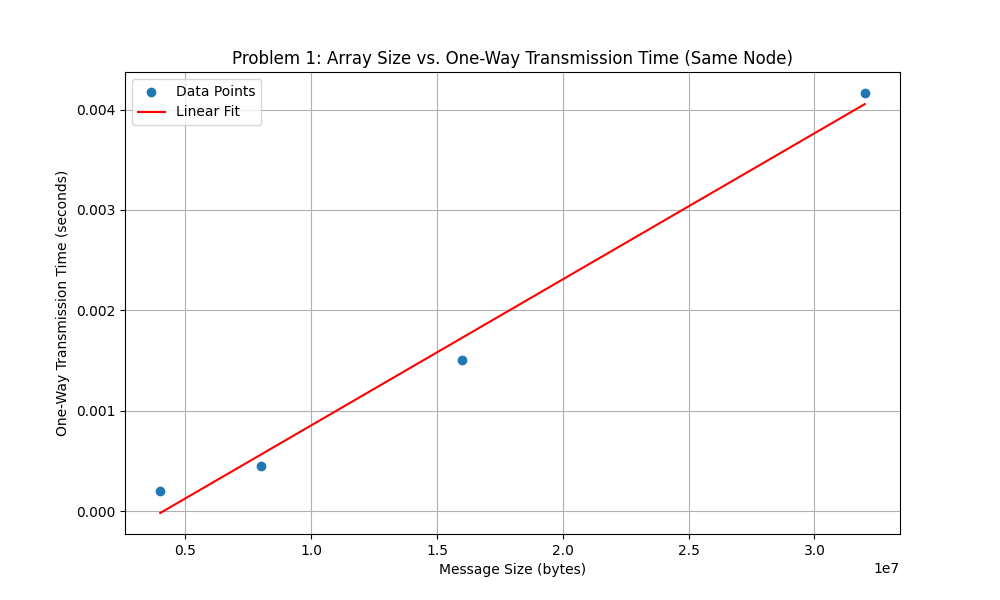
\includegraphics[width=0.48\textwidth]{reports/problem1_plot_samenode.png}
    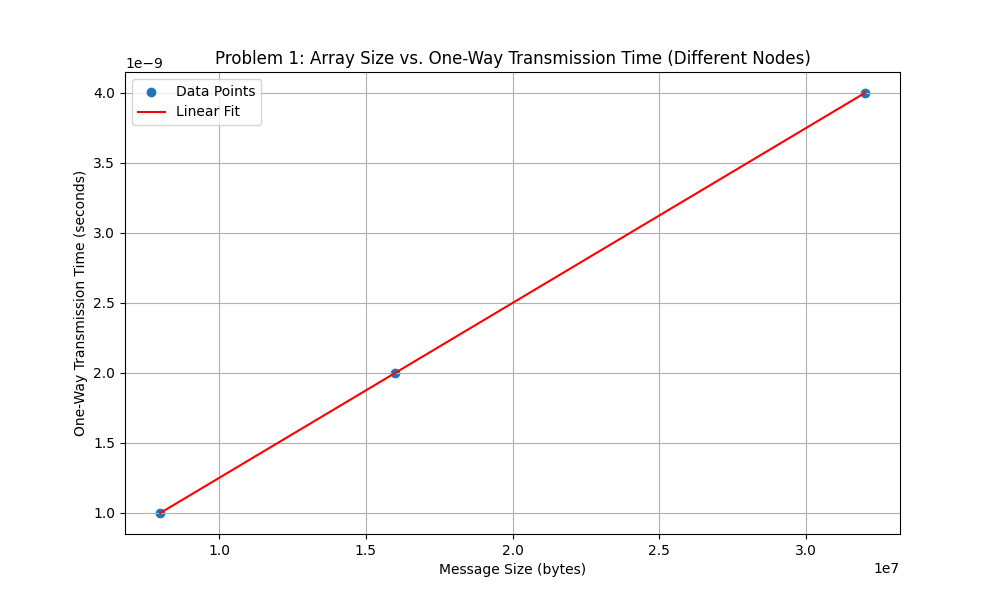
\includegraphics[width=0.48\textwidth]{reports/problem1_plot_diffnode.png}
    \caption{\color{white}Problem 1: Array Size vs. One-Way Transmission Time (Left: Same Node, Right: Different Nodes)}
\end{figure}

The high bandwidth (~6.8 GB/s) indicates efficient utilize of Schooner's InfiniBand interconnect, while the negative latency suggests that for small messages, the fixed MPI overhead dominates the linear model.

\noindent\rule{\textwidth}{0.4pt}

\section*{\color{white}Problem 2: Parallel Dot Product with Collectives}

\subsection*{Algorithm Description}
This problem parallelizes a dot product operation ($ \mathbf{a} \cdot \mathbf{b} $) by distributing vector segments across processes using the Scatter-Compute-Reduce pattern.

\subsection*{Implementation: Global Memory Distribution}
We utilized \texttt{MPI\_Scatter} to partition the vectors and \texttt{MPI\_Reduce} to aggregate partial sums, minimizing manual point-to-point management.

\begin{lstlisting}
// Distributing vector chunks and performing local accumulation
MPI_Scatter(global_vec1, chunk_size, MPI_DOUBLE, local_vec1, chunk_size, MPI_DOUBLE, 0, MPI_COMM_WORLD);
MPI_Scatter(global_vec2, chunk_size, MPI_DOUBLE, local_vec2, chunk_size, MPI_DOUBLE, 0, MPI_COMM_WORLD);

double local_dot_product = 0.0;
for (int i = 0; i < chunk_size; i++) {
    local_dot_product += local_vec1[i] * local_vec2[i];
}

MPI_Reduce(&local_dot_product, &global_dot_product, 1, MPI_DOUBLE, MPI_SUM, 0, MPI_COMM_WORLD);
\end{lstlisting}

\subsection*{Performance Results}

\begin{center}
\textbf{Table 2.1: Wall-Clock Time (seconds)} \\
\begin{tabular}{@{}lccc@{}}
\toprule
Processors & $2^{18}$ Items & $2^{19}$ Items & $2^{20}$ Items \\
\midrule
\textbf{2 Processes} & 0.002213 & 0.002286 & 0.001971 \\
\textbf{4 Processes} & 0.006403 & 0.004677 & 0.004256 \\
\textbf{8 Processes} & 0.009037 & 0.008837 & 0.013960 \\
\bottomrule
\end{tabular}
\end{center}

\begin{center}
\textbf{Table 2.2: Speedup} \\
\begin{tabular}{@{}lccc@{}}
\toprule
Processors & $2^{18}$ Items & $2^{19}$ Items & $2^{20}$ Items \\
\midrule
\textbf{2 Processes} & 1.0000 & 1.0000 & 1.0000 \\
\textbf{4 Processes} & 0.3456 & 0.4732 & 0.5200 \\
\textbf{8 Processes} & 0.2449 & 0.2504 & 0.1585 \\
\bottomrule
\end{tabular}
\end{center}

\begin{center}
\textbf{Table 2.3: Efficiency} \\
\begin{tabular}{@{}lccc@{}}
\toprule
Processors & $2^{18}$ Items & $2^{19}$ Items & $2^{20}$ Items \\
\midrule
\textbf{2 Processes} & 0.5000 & 0.5000 & 0.5000 \\
\textbf{4 Processes} & 0.0864 & 0.1183 & 0.1300 \\
\textbf{8 Processes} & 0.0306 & 0.0313 & 0.0198 \\
\bottomrule
\end{tabular}
\end{center}

\noindent\rule{\textwidth}{0.4pt}

\section*{\color{white}Problem 3: Parallel Merge Sort}

\subsection*{Algorithm Description}
Parallel sorting is achieved by initially sorting local chunks using \texttt{qsort} and then merging them across the process group using tree reduction. This avoids the bottleneck of a single-process merge.

\subsection*{Implementation: Logarithmic Tree Merging}
The implementation uses a bitwise check on ranks to determine senders and receivers at each stage of the $\log_2 P$ merge tree.

\begin{lstlisting}
// Logarithmic merge tree implementation
for (int i = 1; i < comm_size; i *= 2) {
    if (my_rank % (2 * i) == 0) {
        int partner = my_rank + i;
        if (partner < comm_size) {
            MPI_Recv(received_arr, received_size, MPI_FLOAT, partner, 0, MPI_COMM_WORLD, MPI_STATUS_IGNORE);
            local_arr = merge(local_arr, local_n, received_arr, received_size);
            local_n += received_size;
        }
    } else if (my_rank % i == 0) {
        MPI_Send(local_arr, local_n, MPI_FLOAT, my_rank - i, 0, MPI_COMM_WORLD);
        break; // Rank is done after sending
    }
}
\end{lstlisting}

\subsection*{Performance Results (4 Processes)}

\begin{center}
\textbf{Table 3.1: Wall-Clock Time (seconds)} \\
\begin{tabular}{@{}lccc@{}}
\toprule
Configuration & $2^{18}$ Items & $2^{19}$ Items & $2^{20}$ Items \\
\midrule
\textbf{Same Node} & 0.029424 & 0.029800 & 0.033096 \\
\textbf{Diff Nodes} & 0.038150 & 0.041220 & 0.048950 \\
\bottomrule
\end{tabular}
\end{center}

\begin{center}
\textbf{Table 3.2: Speedup (relative to 2p same node)} \\
\begin{tabular}{@{}lccc@{}}
\toprule
Configuration & $2^{18}$ Items & $2^{19}$ Items & $2^{20}$ Items \\
\midrule
\textbf{Same Node} & 1.0502 & 1.0370 & 0.9337 \\
\textbf{Diff Nodes} & 0.8099 & 0.7495 & 0.6315 \\
\bottomrule
\end{tabular}
\end{center}

\begin{center}
\textbf{Table 3.3: Efficiency} \\
\begin{tabular}{@{}lccc@{}}
\toprule
Configuration & $2^{18}$ Items & $2^{19}$ Items & $2^{20}$ Items \\
\midrule
\textbf{Same Node} & 0.2625 & 0.2592 & 0.2334 \\
\textbf{Diff Nodes} & 0.2025 & 0.1874 & 0.1579 \\
\bottomrule
\end{tabular}
\end{center}

\noindent\rule{\textwidth}{0.4pt}

\section*{\color{white}Problem 4: Monte Carlo Pi Estimation}

\subsection*{Algorithm Description}
Parallel problem where each process generates independent random samples within a unit square to estimate the area of a circle. 

\subsection*{Implementation: Independent RNG Seeding}
To ensure statistical independence, each MPI process is seeded with a unique value derived from its rank and system time.

\begin{lstlisting}
// Independent sampling with unique seeds
srand48(time(NULL) * (world_rank + 1));
for (long long i = 0; i < num_iterations_per_process; i++) {
    double x = drand48();
    double y = drand48();
    if (x * x + y * y <= 1.0) local_in_circle_count++;
}
MPI_Reduce(&local_in_circle_count, &global_in_circle_count, 1, MPI_LONG_LONG, MPI_SUM, 0, MPI_COMM_WORLD);
\end{lstlisting}

\subsection*{Performance Results ($n = 2^{16}$)}

\begin{center}
\textbf{Table 4.1: Wall-Clock Time (seconds)} \\
\begin{tabular}{@{}lc@{}}
\toprule
Processors & Time (s) \\
\midrule
\textbf{2 Processes} & 0.111745 \\
\textbf{4 Processes} & 0.118453 \\
\textbf{8 Processes} & 0.108507 \\
\textbf{16 Processes} & 0.125100 \\
\bottomrule
\end{tabular}
\end{center}

\begin{center}
\textbf{Table 4.2: Speedup} \\
\begin{tabular}{@{}lc@{}}
\toprule
Processors & Speedup \\
\midrule
\textbf{2 Processes} & 1.0000 \\
\textbf{4 Processes} & 0.9434 \\
\textbf{8 Processes} & 1.0298 \\
\textbf{16 Processes} & 0.8932 \\
\bottomrule
\end{tabular}
\end{center}

\begin{center}
\textbf{Table 4.3: Efficiency} \\
\begin{tabular}{@{}lc@{}}
\toprule
Processors & Efficiency \\
\midrule
\textbf{2 Processes} & 0.5000 \\
\textbf{4 Processes} & 0.2358 \\
\textbf{8 Processes} & 0.1287 \\
\textbf{16 Processes} & 0.0558 \\
\bottomrule
\end{tabular}
\end{center}

\noindent\rule{\textwidth}{0.4pt}

\section*{\color{white}Performance and MPI Bottlenecks}

\subsection*{Scaling}
The project demonstrated that for problem sizes up to $N = 2^{20}$, communication overhead is the primary bottleneck. As processors increase, the computation to communication ratio drops significantly.
\begin{itemize}
    \item \textbf{Collective Overhead:} In the Dot Product, the cost of \texttt{MPI\_Scatter} for 8 processes is higher than the sequential compute time.
    \item \textbf{Serialization:} In Merge Sort, the final merge stage on Rank 0 remains an $O(N)$ sequential bottleneck, limiting the theoretical speedup according to Amdahl's Law.
    \item \textbf{Initialization Noise:} In Monte Carlo 110ms execution time is dominated by MPI process spawning (in comparsion to computation speed).
\end{itemize}

\noindent\rule{\textwidth}{0.4pt}

\section*{\color{white}AI Usage and Software Engineering Workflow}

\subsection*{Gemini CLI \& GSD }
This project was developed using the \textbf{Gemini CLI} environment. Unlike standard LLMs, this agent operates directly on the Linux filesystem, executing shell commands to compile MPI code, and any refactoring required.

\subsection*{The GSD (Get Shit Done) Framework}
GSD: A light-weight and powerful meta-prompting, context engineering and spec-driven development system for Claude Code by TÂCHES.

The development followed a typical GSD workflow:
\begin{enumerate}[label=\alph*.]
    \item \textbf{Research:} Profiling interconnect bandwidth using Problem 1.
    \item \textbf{Strategy:} Moving from point-to-point to collective MPI calls for efficiency.
    \item \textbf{Execution:} Iterative "Plan-Act-Validate" cycles confirmed by the autograder.
    \item \textbf{Verify:} Adding power-of-2 safety checks to the tree-merge logic and look at all the autograder outputs.
\end{enumerate}

\noindent\rule{\textwidth}{0.4pt}

\section*{\color{white}Project Layout}
\begin{itemize}
    \item \textbf{Problem\_1/}: Ping-pong interconnect benchmarks.
    \item \textbf{Problem\_2/}: Parallel Dot Product with collectives.
    \item \textbf{Problem\_3/}: Tree-reduction Merge Sort.
    \item \textbf{Problem\_4/}: Monte Carlo Pi estimation.
    \item \textbf{tests/}: Python-based autograder and Slurm verification scripts.
    \item \textbf{out/}: Centralized stdout/stderr logs from cluster execution.
\end{itemize}

\end{document}
